\documentclass[dutch, a4paper, 11pt]{article}
\usepackage[utf8]{inputenc}

%Margins 
\usepackage[a4paper, left=1.27cm,top=1.27cm,right =1.27cm, bottom = 1.4cm]{geometry}

%Load packages
%Algemene packages
\usepackage{babel}
\usepackage{slantsc}
\usepackage{array}
\renewcommand{\arraystretch}{2}
\usepackage{multicol}
\usepackage{multirow}
\usepackage{amsmath}
\usepackage{amsfonts}
\usepackage{booktabs}

%Opsommingen
\usepackage{enumerate}


%Afbeeldingen
\usepackage{graphicx}
\usepackage{wrapfig}

%Gekleurde tekstboxen 
\usepackage[most]{tcolorbox}

%Stop indent
\setlength{\parindent}{0pt}

%Font
\usepackage{cmbright}
\usepackage[OT1]{fontenc}

%Headers and footers
\usepackage{fancyhdr}

\pagestyle{fancy}
\fancyhf{}
\renewcommand{\headrulewidth}{0pt}
\renewcommand{\footrulewidth}{0pt}
\fancyhead[LE,RO]{}
\fancyhead[RE,LO]{}

%Logo in footer
\usepackage{lastpage}
\lfoot{}
\cfoot{\vspace{-5mm} \thepage}
\rfoot{}

%Voorbeeldtekst
\usepackage{lipsum}

%Meerdere kolommen
\usepackage{multicol}
\setlength{\columnsep}{1cm}

%Whitespace na section
\usepackage[compact]{titlesec}  
\titlespacing{\section}{0pt}{2pt}{0pt}

%Tekst kleur
\usepackage{xcolor}

%Nieuwe kleur
%\definecolor{ugent_blue}{rgb}{0.04706, 0.13725, 0.26667}
\definecolor{ugent_blue}{RGB}{30, 100, 200}

%Nummering sections
\renewcommand\thesection{\arabic{section}}
\renewcommand\thesubsection{\thesection.\arabic{subsection}}

%Lay-out hoofdingen
\titleformat*{\section}{\bfseries \normalfont}
\usepackage{sectsty}
\sectionfont{\color{ugent_blue}}
\titlespacing\section{0pt}{10pt plus 4pt minus 4pt}{0pt plus 2pt minus 2pt}

\raggedbottom


%other shit that may be useful
\usepackage{multicol,caption}
\usepackage{mathtools}
\raggedbottom
\newcommand{\HRule}{\hrule}
\abovedisplayskip0pt
\renewcommand{\arraystretch}{1.5}
\newcolumntype{M}[1]{>{\centering\arraybackslash}m{#1}}
\usepackage{lscape}
\newenvironment{Figure}
  {\par\medskip\noindent\minipage{\linewidth}}
  {\endminipage\par\medskip}
\usepackage{float}
\usepackage{hyperref}
\newcommand\myfigure[1]{%
\medskip\noindent\begin{minipage}{\columnwidth}
\centering%
#1%
%figure,caption, and label go here
\end{minipage}\medskip}
\usepackage{caption}
\usepackage{subcaption}
\usepackage{tabularx}
\usepackage{enumerate}
\usepackage{enumitem}

\raggedbottom
\raggedcolumns




\begin{document}

%Load heading of document
%ugent color
{\color{ugent_blue} \hrule\hrule\hrule}

\vspace*{-0.43mm}
\colorbox{ugent_blue}{\color{white} \bf Report Biomechanics}\\

\noindent\begin{minipage}{0.7\textwidth}% adapt widths of minipages to your needs
{\LARGE \bf \color{ugent_blue} Clinical Movement Analysis Lab Assignment 2022}\\[2mm]

%
{\large Vincent Belpaire}\\
{Supervisor: Prof. Malcolm Forward}\\


{\small University of Ghent}\\
{\small Faculty of Engineering and Architecture}\\
{\small Bachelor of Science: Biomedical Engineering}\\
\end{minipage}%
\hfill%
\begin{minipage}{0.3\textwidth}
\vspace{-2.2cm}
\begin{center}

\includegraphics[width=\linewidth]{ugent_logo}
\end{center}
\end{minipage}\\


\begin{tcolorbox}[colframe=ugent_blue, colback=ugent_blue!10, enhanced jigsaw, boxrule=0.5pt]
{\bf Abstract}\\
A well made report of an experiment is crucial in research. It should contain all necessary information so if one would read
it again a couple of years after the execution of the experiment one could redo it without many errors. In short, the report 
must allow repetition. This is only possible if all used parameters and methods are mentioned. And as a check, the results and
conclusions should also be displayed.\\
This little article contains three reports. Each report relates to one of the practicals done at UZ Gent Campus: NTA, 3D cell culture and H\&E. 
\end{tcolorbox}


%Start writing your repot...

\begin{multicols}{2}  %Write in two columns

%%%%%%%%%%%%%%%%%%%%%%%%%%%%%%%%%%%%%%%%%%
%Section 1
%%%%%%%%%%%%%%%%%%%%%%%%%%%%%%%%%%%%%%%%%%

\section{NTA, Nanoparticle Tracking Analysis}

\subsection{aim}

Calculating the size and concentration of particles in scatter and fluorescent mode for EV-characterisation.

\subsection{material and methods}

An LM10-series microscope, which utilizes the principles of light scattering and Brownian motion, was used to visualize the particles in the sample as highlighted points with highlighted tails. With the \emph{NTA 3.4 - Sample Assistant Build 3.4.4 - SA} software the concentration and size distribution were calculated.\\
Two types of samples were used. Both samples were rEVs but one had a scatter mode (SM) pre-treatment and one a fluorescent mode (FM) pre-treatment. Table \ref{T1} displays the environmental settings for both types of pre-treatments. All samples were made in a diluent of $\frac{1}{8000}$.

\begin{table}[H]
\scalebox{0.7}{\begin{tabular}{c|c|c}
& scatter mode & fluorescent mode\\
\hline
Temperature/C & $21.40-21.50$ & $21.90-22.0$\\
Viscosity/cP & $0.966682-0.964370$ & 0,$95521-0,952941$\\
Camera Type & sCMOS & sCMOS\\
Laser Type & Blue488 & Blue488\\
Camera Level & $13$ & $16$\\
Syringe Pump Speed/AU & $20$ & $20$\\
Detection Threshold & $3$ & $3$\\
\end{tabular}}
\caption{Environmental settings}
\label{T1}
\end{table}

For each treatment type three videos were recorded.

\subsection{results and discussion}

Only the concentrations in particles per ml are displayed. To have the absolute particle concentration, 
i.e. the absolute particle count, these concentrations should be multiplied with 8000 ml.\\
Table \ref{T2} shows the concentrations of different treatment-types. Using the averages of SM and FM to 
calculate the ratio of fluorescent particles gives $\frac{7,57\text{E+}08}{8,61\text{E+}08}= 0.879$.
A high ratio indicates a well-executed seperation in the EV-seperation phase prior to the EV-characterisation which is the case in this experiment.

\begin{table}[H]
    \scalebox{0.7}{\begin{tabular}{c|c|c|c|c|c}
    & video 1 & video 2 & video 3 & mean & standard error\\
    \hline
    SM & 8,14E+08 & 8,69E+08 & 9,00E+08 & 8,61E+08 & 2,53E+07\\
    FM & 7,51E+08 & 7,51E+08 & 7,45E+08 & 7,57E+08 & 9,17E+06
    \end{tabular}}
    \caption{concentrations (particles/ml)}
    \label{T2}
    \end{table}

    Figures \ref{F1} and \ref{F2} displays repsectively the size distribution of the different SM and FM samples.

\vspace*{-0.5cm}
\begin{figure}[H]
    \centering
    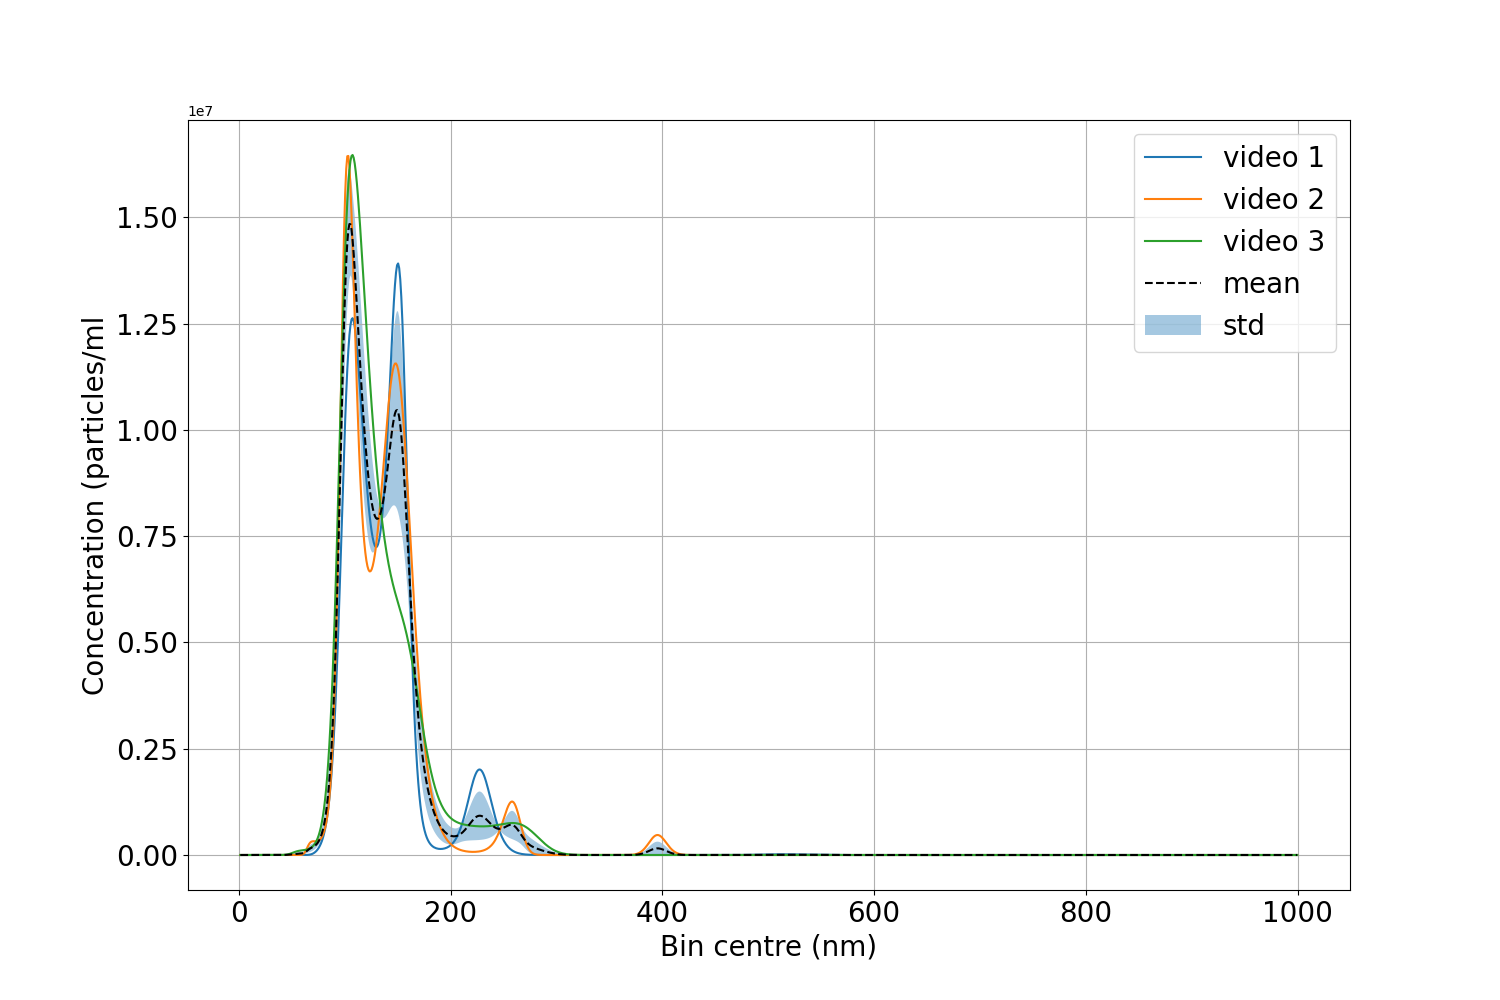
\includegraphics[scale=0.2]{fig_scatter.png}
    \caption{Size distribution - scatter}
    \label{F1}
\end{figure}
\vspace*{-0.5cm}
\begin{figure}[H]
    \centering
    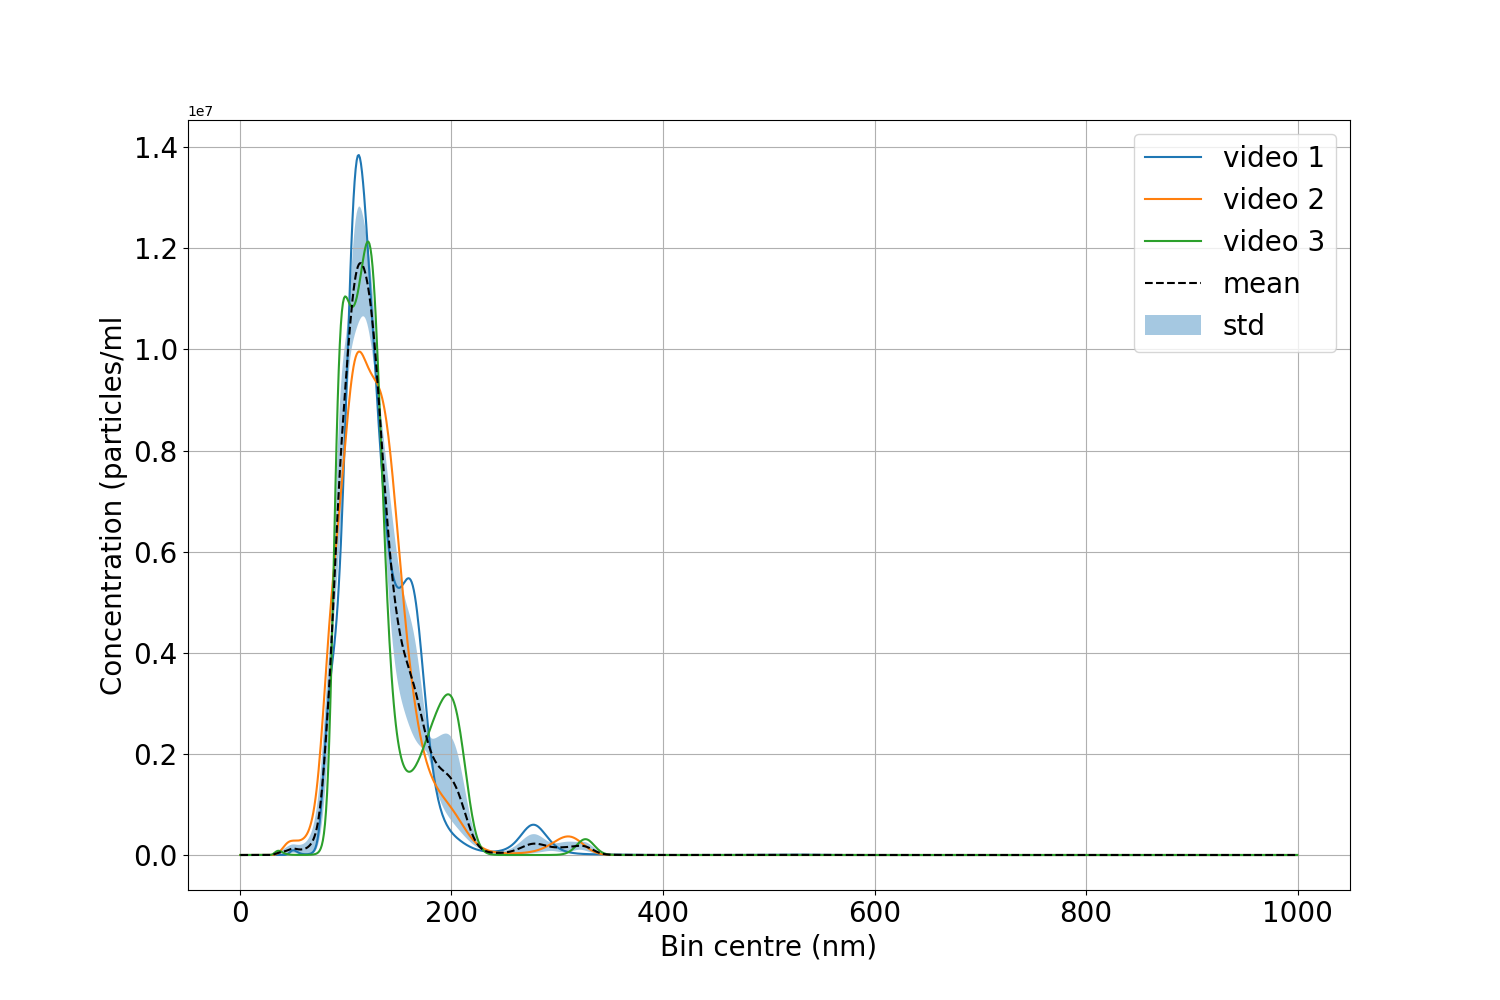
\includegraphics[scale=0.2]{fig_fluo.png}
    \caption{Size distribution - fluorescent}
    \label{F2}
\end{figure}

\subsection{conclusion}

NTA allows the researcher to analyse a relatively high resolution of particles and with the use of
fluorescense makes it possible to score the EV-seperation.

%%%%%%%%%%%%%%%%%%%%%%%%%%%%%%%%%%%%%%%%%%
%Section 2
%%%%%%%%%%%%%%%%%%%%%%%%%%%%%%%%%%%%%%%%%%

\section{3D cell culture}

\subsection{aim}

Analysing the size and morphology of 3D cell cultures for groups with high glucose (HG)
and low glucose (LG) and compairing them statistically.

\subsection{material and methods}

The following steps were executed on a given data set of tiff-files.\\
ImageJ was used to determine the pixel to micrometer conversion which gave as result that 
$500$ $\mu$m  corresponds to $313$ pixels, hence $1$ pixel $=\frac{500}{313}\mu$m.\\
With AnaSP data was extracted from the tiff-files. This data contains several parameters whereof two were chosen, 
\emph{Circularity} and \emph{FeretDiameterMax}, for a statistical compairinson between the two groups (LG and HG).
These two parameters were chosen because the shape, as \emph{Circularity}, is compaired as well as the size, as \emph{FeretDiameterMax}.\\
In the statistical analysis a significance level of $5\%$ was used. For both parameters a independent t-test
was perfomed to compaire if their means are equal, null hypothesis, or significanlty different, alternative hypothesis.\\
Note that to use the independent t-test, homoscedasticity must be fulfiled.

\subsection{results and discussion}

In figure \ref{fig:t-test} (look at end of this article) the results of the independent t-tests are listed. For the \emph{FeretDiameterMax} there is no significant dfference, hence the null hypothesis for this 
parameter was accepted. This implies that the size of the cell can not be used to distinct between groups.\\
For the \emph{Circularity} the condition of homoscedasticity is not fulfilled thus the results of the t-test can not be used. But if homoscedasticity is not fulfilled in the first place then
must there be a significant difference between the two groups, hence Circularity is a good parameter to distinct both groups from each other.

\subsection{conclusion}

Some parameters are good for distinction between groups while others are not. With the 
appropriate software tools it is possible to determine which parameters are suitable for this role.

%%%%%%%%%%%%%%%%%%%%%%%%%%%%%%%%%%%%%%%%%%
%Section 3
%%%%%%%%%%%%%%%%%%%%%%%%%%%%%%%%%%%%%%%%%%

\section{H\&E, Hematoxylin/Eosin staining}

\subsection{aim}

Analysing 2 slides from mice tissue for their structural composition by identifying their tissue type and occurring structures.

\subsection{material and methods}

The slides were prepared using the standard H\&E method at the UZ Gent campus which will not be discussed in this report.\\
The name of the method refers to the two used stains, i.e. hematoxylin and eosin. Hematoxylin has a purple color and binds to the nucleus while eosin is rather pinkish and remain in the cytoplasm.

\subsection{results and discussion}

Figure \ref{fig:Mt} displays muscle tissue. Three regions are indicated as I, II and III and have the following observations:
\begin{itemize}
    \item[I] skeletal muscle
    \item[II] fat tissue
    \item[III] tumorous tissue
\end{itemize}

\begin{figure}[H]
    \centering
    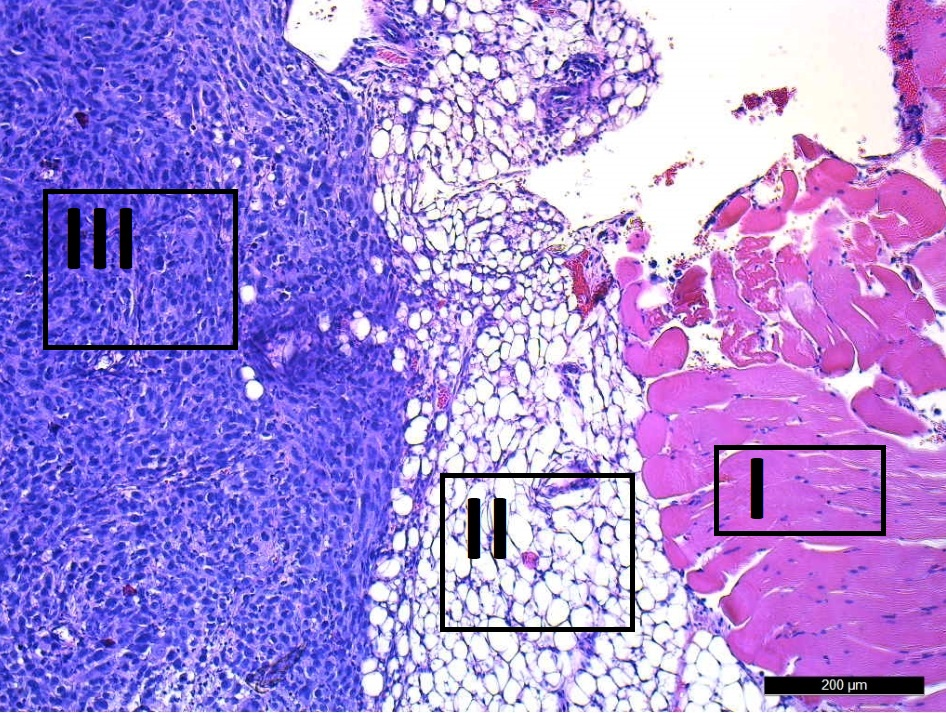
\includegraphics[scale=0.4]{H&E 02}
    \caption{Muscle tissue}
    \label{fig:Mt}
\end{figure}

Figure \ref{fig:Mt} displays kidney tissue. The two circles, indicated with I, are glomeruli of the kidney.

\begin{figure}[H]
    \centering
    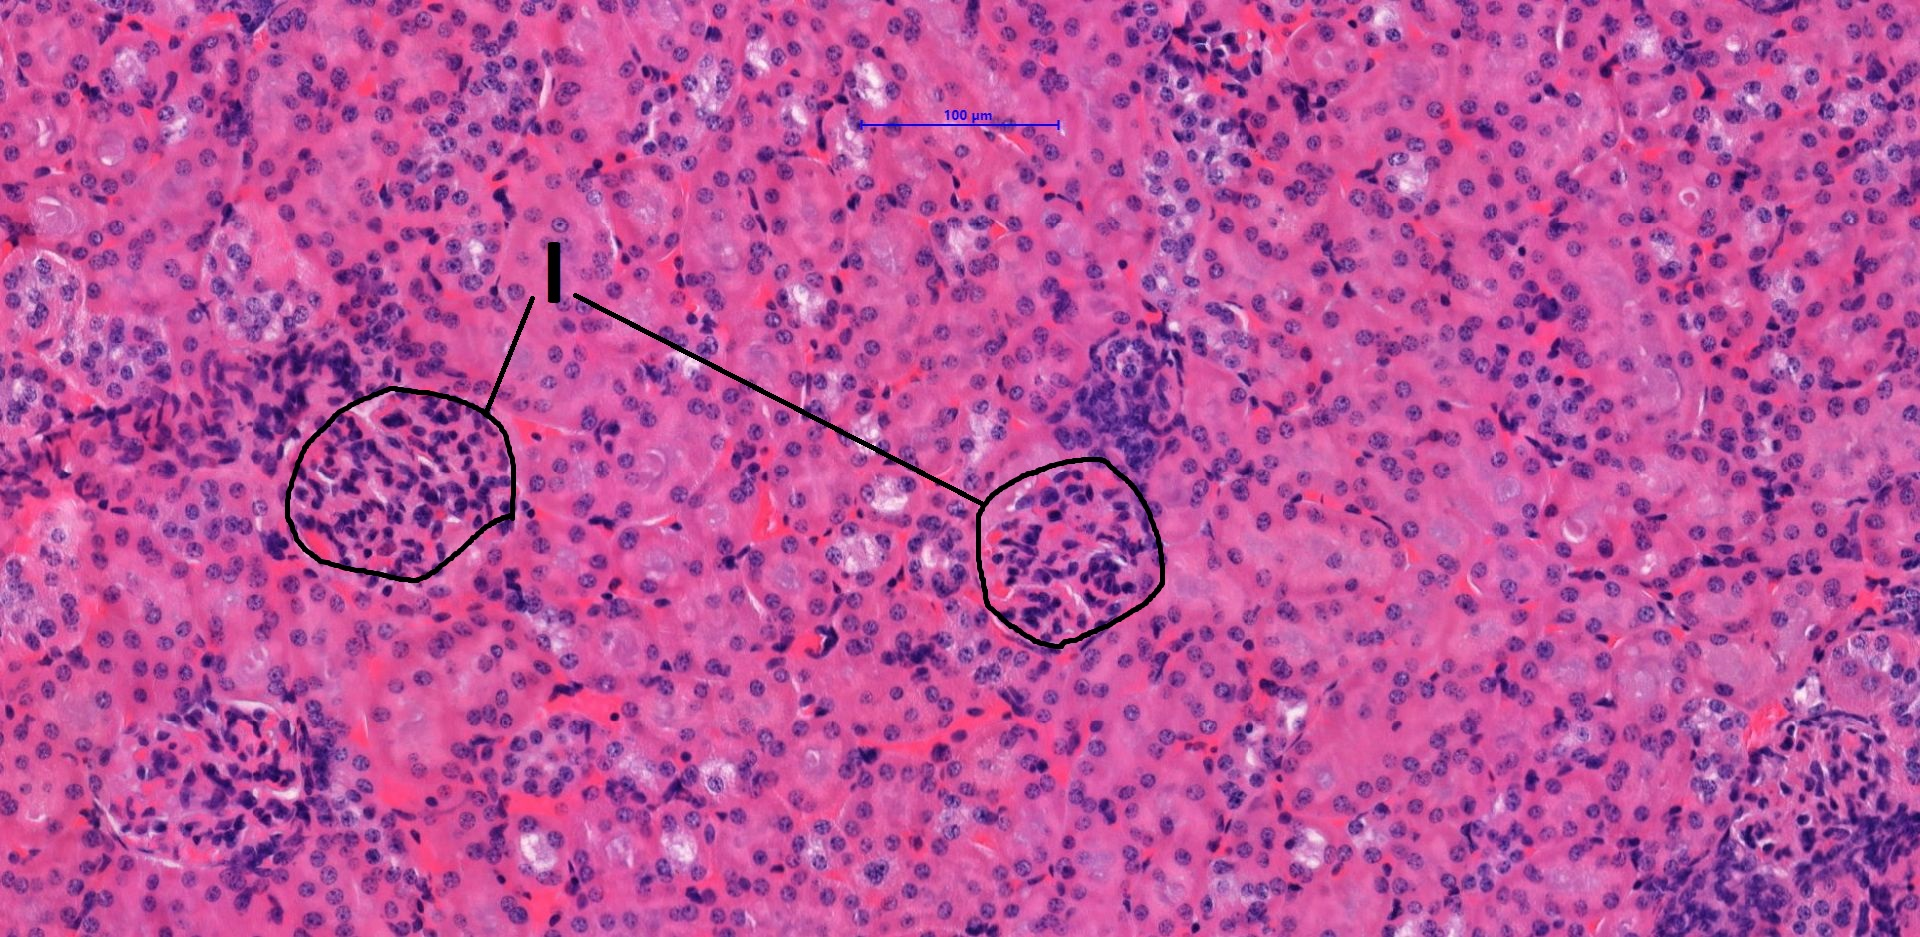
\includegraphics[scale=0.15]{H&E 12}
    \caption{Kidney tissue}
    \label{fig:Kt}
\end{figure}

\subsection{conclusion}

With H\&E staining it is possible to visualize tissue structures so that it can be analysed by humans via a microscope.
Besides the clear images presented, there is steel need of expertise to have good indetification of the different components.
It is not allways clear to identify the different tissue structures and if tissue of an ill-subject would be analysed it would get 
even more challenging.

\end{multicols}

\section{SPSS output}

\begin{figure}[H]
    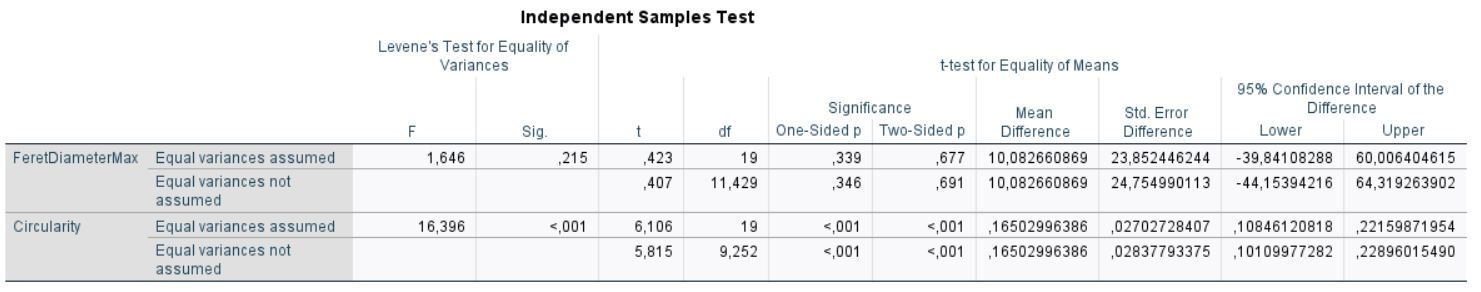
\includegraphics[scale=0.6]{outpt_t_test.png}
    \caption{Independent t-test results}
    \label{fig:t-test}
\end{figure}


\end{document}
